\documentclass[a4paper,11pt]{article}
\usepackage[utf8]{inputenc}
\usepackage{graphicx}
\usepackage[english]{babel}
\usepackage[vmargin=3.5cm, top=2cm]{geometry}
\usepackage[linktocpage=true]{hyperref}
\usepackage{enumitem}
\usepackage{longtable}
\usepackage{pdfpages}
\usepackage{float}
\usepackage{hyperref}
\usepackage[section]{placeins}
\hypersetup{
   colorlinks,
   citecolor=black,
   filecolor=black,
   linkcolor=black,
   urlcolor=black
}

\begin{document}

\begin{titlepage}

\centering \parindent=0pt
\newcommand{\HRule}{\rule{\textwidth}{1mm}}
\vspace*{\stretch{1}} \HRule\\[1cm]\Huge\bfseries
Data Mining Report\\[0.7cm]
\HRule\\[4cm]  
\large by 
\\ Mikkel Stolborg
\\ Hlynur Örn Haraldsson
\vspace*{\stretch{2}} \normalsize %
\begin{flushleft}
IT University of Copenhagen \\
MDMI, S2015\\
Anders Hartvig Hartzen\\
Hajira Jabeen\\
Héctor Pérez Martínez\\
Sebastian Risi\\
Noor Shaker\\
\today 
\end{flushleft}
\end{titlepage}

\tableofcontents
\pagebreak
%\section{Introduction}
%This report deals with data mining on data gathered about the passengers on the titanic. The primary idea is to figure out if there is any relation between the variables as to who survived. We primarily 

%First we will discuss the data selection, the research question of this report, and go over the tools used.

%We will then go through the data mining process, the methods used and analyse the outcome.  It is also in this section we will go through the preprocessing.

%Finally we will conclude upon the project and see if there is any societal impact from our data analysis.
%\clearpage
\section{Data selection}
We have worked on a data set regarding the passengers on the titanic. The data structure is presented in table \ref{titanData} with a short name and the value type associated with the variable.
\begin{table}[h]
\begin{tabular}{|l|l|l|}
\hline
Variable name & Short name & Value Type\\
\hline
survival & Survived & binary\\
pclass & Passenger Class & numeric\\
name & Name & string\\
sex & Sex & binary string\\
age & Age & numeric\\
sibsp & Number of Siblings/Spouses Aboard & numeric\\
parch & Number of Parents/Children Aboard & numeric\\
ticket & Ticket Number & string\\
fare & Passenger Fare & numeric\\
cabin & Cabin & string\\
embarked & Port of Embarkation & attribute table\\
\hline
\end{tabular}
\caption{Titanic data set variables with short description and classification.}
\label{titanData}
\end{table}

The type binary and binary string, means there is only two options, the first of the types is based on numeric binary data, whilst the second is based on string data. The value type attribute table covers three options. The type designation in the table are based on how they are treated in the data mining code. This means that whilst some of the other variables might be a three option choice, it will not be treated as such. The reason for this division is mostly due to the nature of string variables and numeric variables.

\subsection{Data description}
The variables in the table are specified as follows. 

Survival is simply a 1 for survived and 0 for not. 

Passenger Class is a numeric value which can take on either 1, 2, or 3. The lower the value, the higher the class. The class is a proxy for the passengers socio-economic status.

Name is simply the name of the passenger, starting with surname.

Sex is the sex of the passenger.

Age is the age in years of the passenger. If the age is less than one it is fractional, and if it is estimated the age is in the form xx.5, meaning it has a decimal value as well.

Number of Siblings/Spouses Aboard, is the number of relatives, yet some of the relations are ignored. The meaning of sibling and spouse is summarized below.

Number of Parents/Children Aboard, is similar to the Number of Siblings/Spouses Aboard. The meaning is as well summarized below.
\begin{itemize}
	\item[\textbf{Sibling:}] Brother, Sister, Stepbrother, or Stepsister of Passenger Aboard Titanic
	\item[\textbf{Spouse:}] Husband or Wife of Passenger Aboard Titanic (Mistresses and Fiances Ignored)
\item[\textbf{Parent:}] Mother or Father of Passenger Aboard Titanic
\item[\textbf{Child:}] Son, Daughter, Stepson, or Stepdaughter of Passenger Aboard Titanic
\end{itemize}

Other family relatives excluded from this study include cousins, nephews/nieces, aunts/uncles, and in-laws.  Some children travelled only with a nanny, therefore parch=0 for them.  As well, some travelled with very close friends or neighbours in a village, however, the definitions do not support such relations.

Ticket Number is the number printed on the ticket. It is basically an identification string with characters and numbers. The tickets have no real pattern.

Passenger Fare is how much the passenger paid for its ticket. The price probably is listed in dollars.

Cabin is the cabin number. Again this is an identification of the rooms, yet there is not really any good patterns within the identification string.

Port of Embarkation is the place of embarking for the passenger. The port is abbreviated as follows. C is for Cherbourg,	Q is for Queenstown, S is for Southampton.

\subsection{Research question}
Our primary question which we want answered was:\\
\textit{"Which attributes contributes mostly to the survival rate of a passenger on the Titanic}\\
Here we wished to figure out what set of parameters would ensure the highest rate of survival on the Titanic. We would use classification through a classification tree to figure out which set gives the highest percentage of survival.

The secondary question arose when looking at clusters of the data.\\
\textit{"Which societal data can be found in clusters of the titanic data"}\\
Looking at the data, we decide to try clustering to see if there was an emergent pattern. It would be interesting to see if the were a relation between wealth and number of children and the like. 
\subsection{Tools for data mining}
We choose to use the free tool called Orange\cite{orange}. This tool allowed to quickly manipulate the data, such that we could extract the interesting elements. 
In the tool you manipulate the data by clicking and drawing connections between data elements and processing methods. Before explaining further, we have included the map of the process used for our data set in the orange framework, see figure \ref{OrangeMap}. The figure presents a brief overview of the data mining process, a better image of the individual parts will be presented in their appropriate sections. 
\begin{figure}[h]
	\centering
	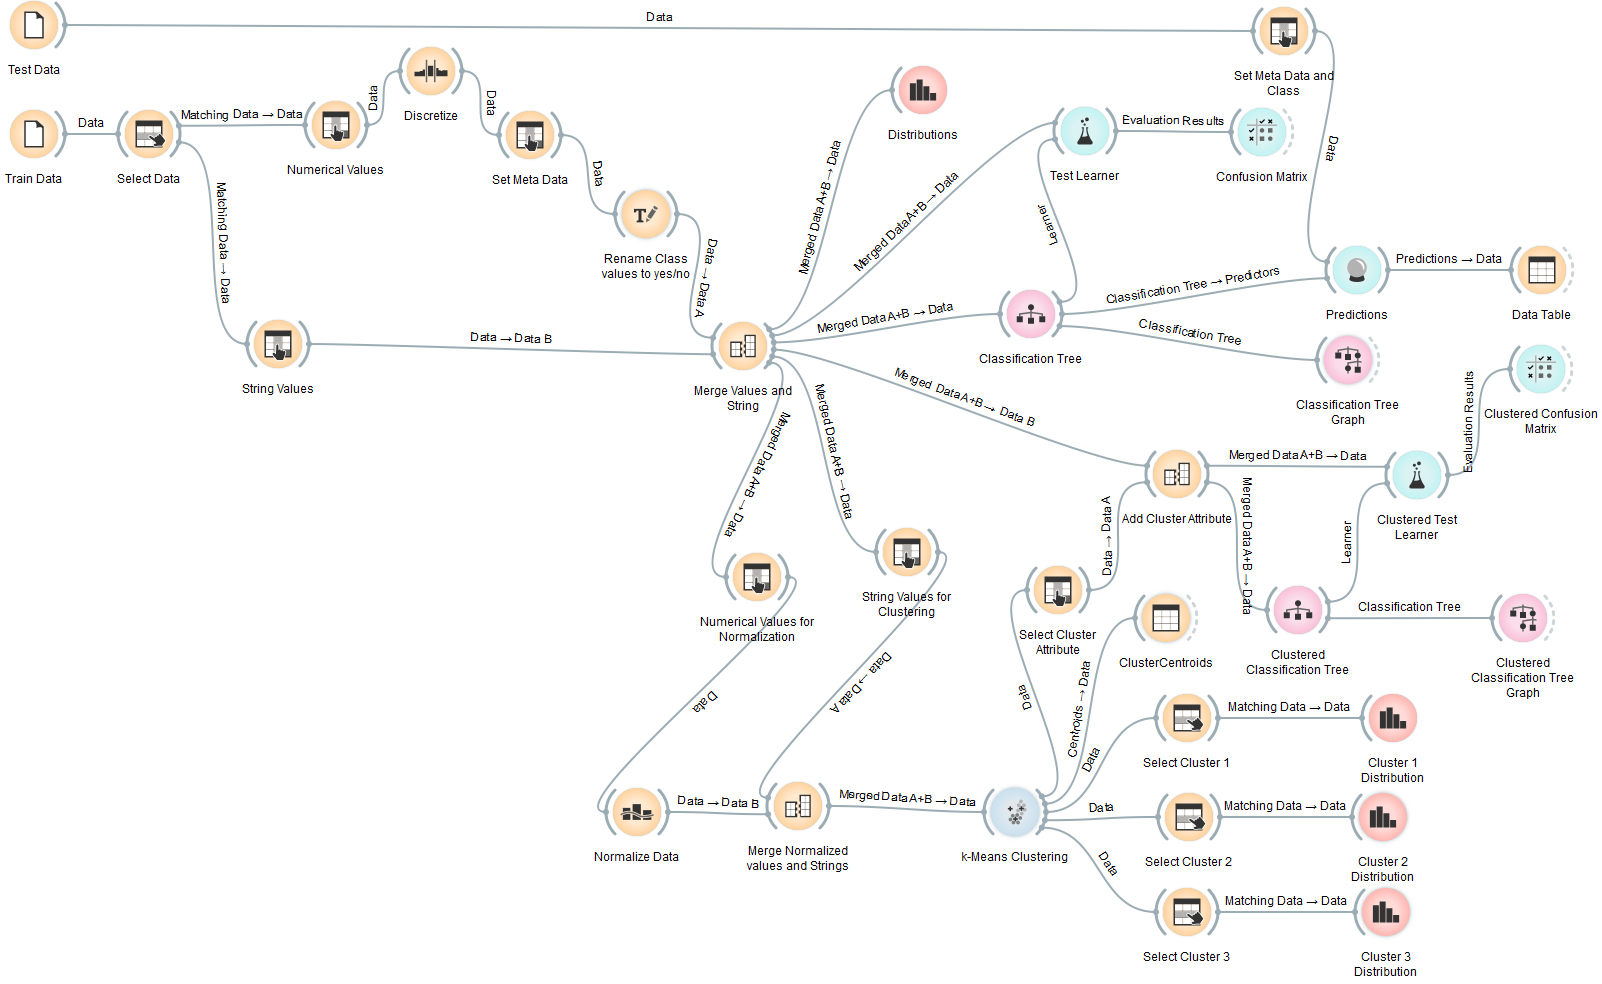
\includegraphics[scale=0.35]{orangeMap}
	\caption{The map of the methods and processes used on the data.}
	\label{OrangeMap}
\end{figure}

\clearpage
\section{Data mining}
This section goes through the data mining process, detailing the methods used and analysing and explaining the output. 
\subsection{Preprocessing}
The data input we got from Kaggle\cite{kaggleData}, was quite neat and easy to work with. This lead to very little preprocessing and general expectation of functioning data. 
However some of the data, even though extensive, had no sensible patterns from which information could be unlocked, and some data were discarded as they were not directly related to our research question. 
We choose to remove the Ticket Number from our data set, as there were no easily identifiable pattern and there were many missing values. The same arguments were used to remove the cabin data. 
The Name of the passengers were discarded as well, as it was not interesting in the methods we choose to apply to the data. 

The main reduction in entries in our data, rather than attributes, were to remove any entry with missing attributes. There was removed 182 entries, mainly due to lack of age, whilst a few, 2, were removed because of lacking Embarked. 
A small reduction in data were made to remove outliers in respect to fare, simply because their presence simply deteriorate the remaining data. This can be supported by looking at the Fare distribution before any preprocessing has been done, see figure \ref{farepreprocess}.

\begin{figure}[h]
\begin{center}
	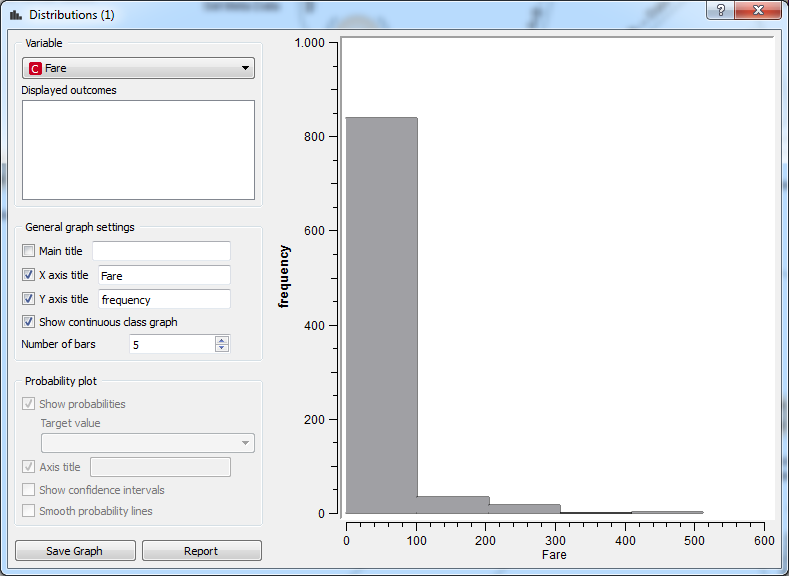
\includegraphics[scale=0.6]{FarePreprocess}
\end{center}
\caption{Fare distribution on initial dataset. The black area between 300 and 400, indicates no persons.}
\label{farepreprocess}
\end{figure}

From the figure it is clear that the outliers of the 3 people who paid more than 400. Removing the outliers gives a more detailed view of the inter relations of the other values.

The total process in the orange framework can be seen in figure \ref{preprocessMap}. The discretize function is there to tell the orange frame work that the survival data is indeed discrete data. The meta data in this case is the passenger id, which is used for merging throughout the framework. Finally the discrete values of the survival variable is being renamed to "yes" and "no". The data is merged and sent out for further use.

\begin{figure}
	\begin{center}
	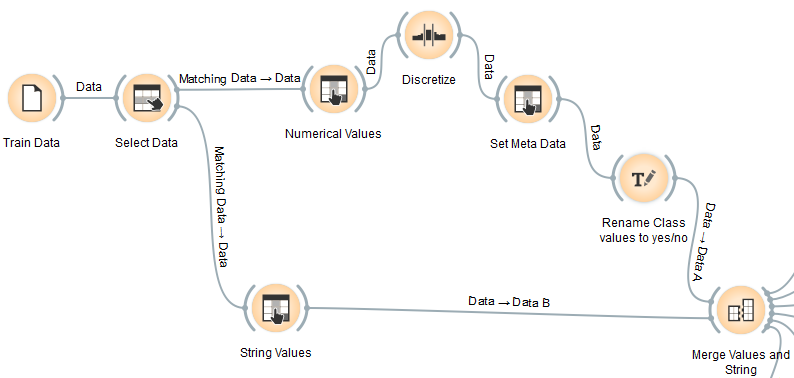
\includegraphics[scale=0.7]{PreprocessMap}
	\end{center}
	\caption{Orange map of preprocessing. The data is prepared for the algorithms and unnecessary data is removed.}
	\label{preprocessMap}
\end{figure}

\subsection{Classification tree}
The classification tree is built upon the information gain of the attributes give to it. The information gain lets us known on which attribute the tree should split upon.
\subsubsection{Implementation}
With the classificat 
\subsubsection{Cross Validation}
10 fold Cross validation
\subsection{K-means Clustering}
K-Means clustering\cite{KMeans} works by first defining K number of clusters, then you feed normalized data to the clustering algorithm, the algorithm chooses K-initial centroids and starts calculating the distance to each data point and then clusters the data around those centroids. After each loop the centroid is recalculated in accordance to all data points in cluster and then the algorithm recalculated the distance to every point. This loop continues until the algorithm runs its loop once without changing anything or is within the minimal change value.
\subsubsection{Implementation}
We decided to use K-Means Clustering in order to increase the accuracy of our Classification Tree by adding the clusters to the attribute of the original data.

How ever after reclassifying with the clusters as an extra attribute we saw that it did not increase accuracy as expected. After looking into the clustered data we saw that the clustering and the classification focused on the same attributes so that did not help us in increasing accuracy.

How ever while looking over the clusters we could see interesting facts about the clusters and were able to find connections regarding clusters.

For example we saw that in cluster 1, every person there was male, mostly lower class, most of them paid under 20 dollars for their Fare and almost all of them embarked from Southampton(S).

How ever if we look at Cluster 3, that cluster is mostly male, mostly upper class and most of them embarked from Cherbourg(C).

What we can extract from this data is, that if you were upper class you would most likely be living in Cherbough.
We can also see that people living in Cherbourg and Queenstown(Q) generally had more money than people living in Southampton. If we look at the fare graph difference between Cluster 1 and 3 we can see a big difference, people living in Southampton would generally pay less than 20 dollars for the ticket and almost no one paid more than that. How ever in Cluster 3 we can see that people still mostly paid under 20 dollars however we can also see that there are a lot more people willing to pay more than the 20 dollars.

\begin{table}[h]
\begin{tabular}{|l|l|l|l|l|l|l|}
\hline
Sex & Embarked & Class & Age & Sibling/Spouse & Parent/Children & Fare\\
\hline
Male & S & 2.428 & 30.28 & 0 & 0 & 21.5697\\
Female & S & 2.258 & 26.32 & 1 & 1 & 35.2690\\
Male & C & 1.552 & 34.14 & 0 & 0 & 66.8577\\
\hline
\end{tabular}
\caption{Cluster Centroids after clustering.}
\label{clusterCentroids}
\end{table}

\begin{figure}[h]
	\centering
	\begin{center}
		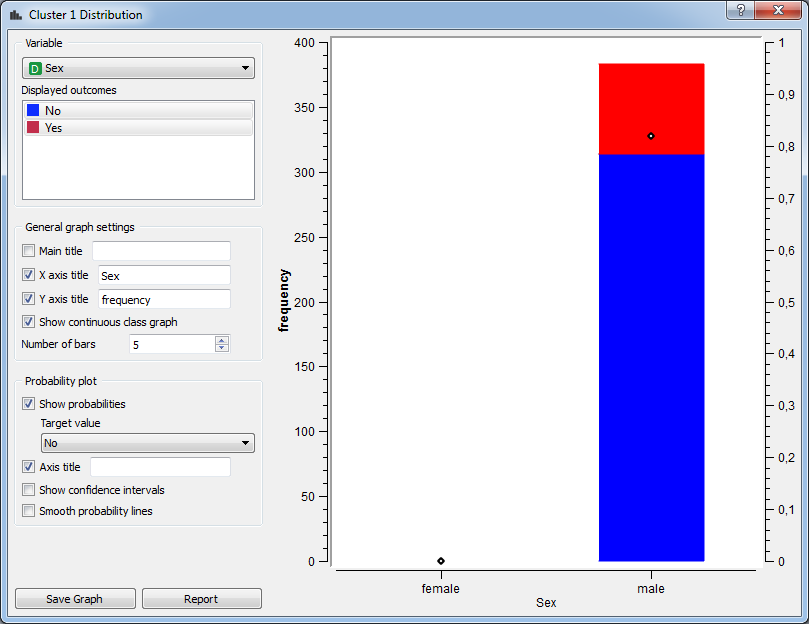
\includegraphics[scale=0.30]{ClusterDistribution/Cluster1/Sex}
		\includegraphics[scale=0.30]{ClusterDistribution/Cluster1/PClass}\\
		\vspace{1 mm}
		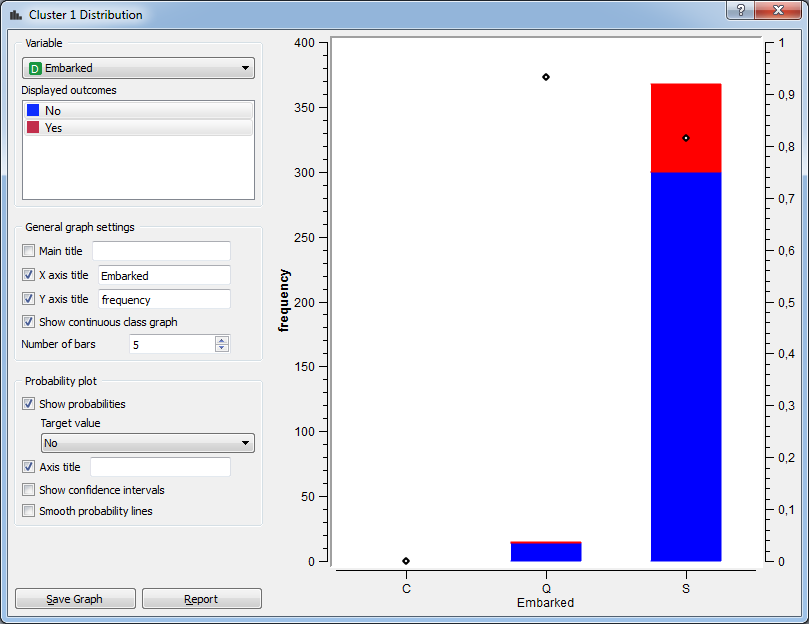
\includegraphics[scale=0.30]{ClusterDistribution/Cluster1/Embarked}
		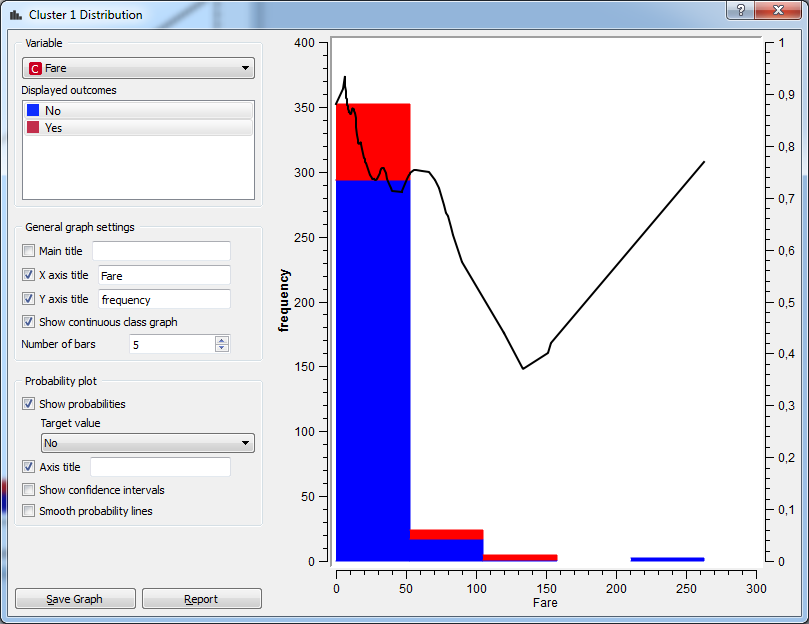
\includegraphics[scale=0.30]{ClusterDistribution/Cluster1/Fare}
	\end{center}
	\caption{Cluster 1}
	\label{ClusterOne}
\end{figure}

\begin{figure}[h]
	\centering
	\begin{center}
		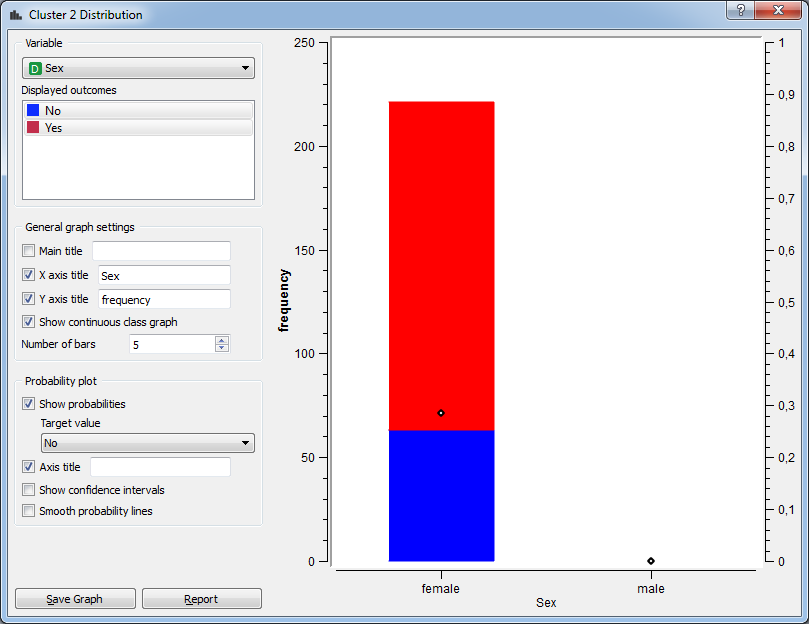
\includegraphics[scale=0.30]{ClusterDistribution/Cluster2/Sex}
		\includegraphics[scale=0.30]{ClusterDistribution/Cluster2/PClass}\\
		\vspace{1 mm}
		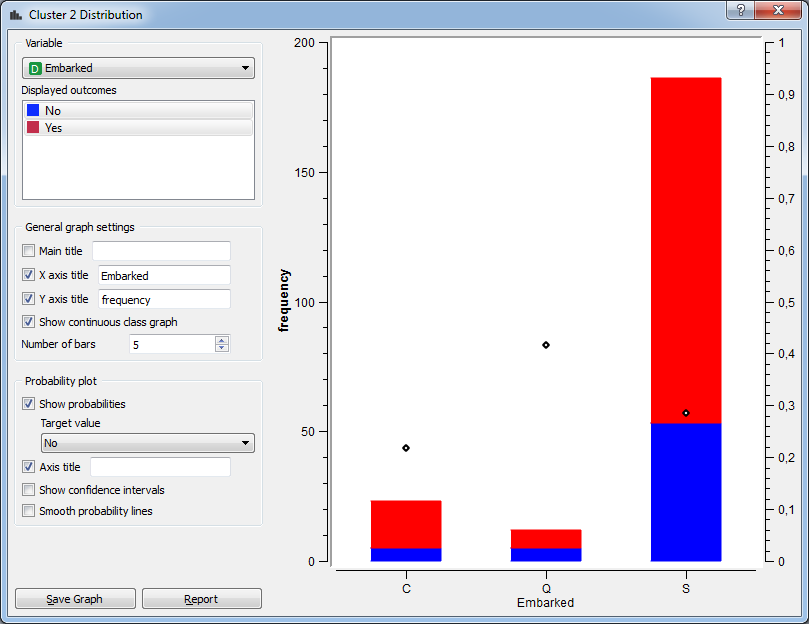
\includegraphics[scale=0.30]{ClusterDistribution/Cluster2/Embarked}
		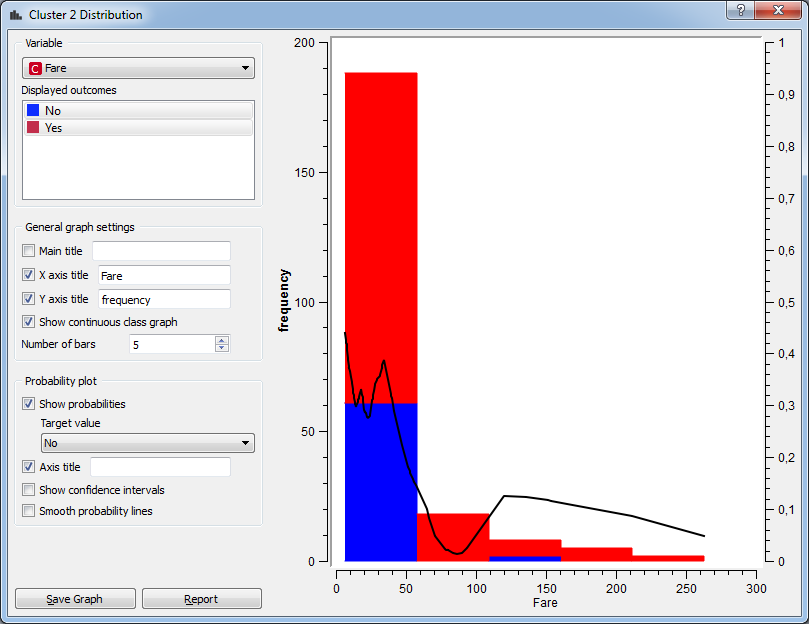
\includegraphics[scale=0.30]{ClusterDistribution/Cluster2/Fare}
	\end{center}
	\caption{Cluster 2}
	\label{ClusterTwo}
\end{figure}

\begin{figure}[h]
	\centering
	\begin{center}
		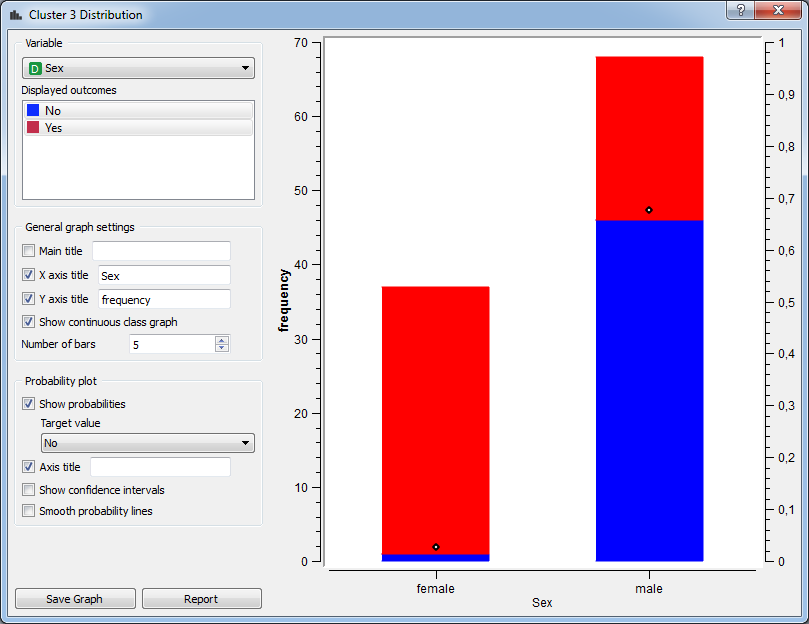
\includegraphics[scale=0.30]{ClusterDistribution/Cluster3/Sex}
		\includegraphics[scale=0.30]{ClusterDistribution/Cluster3/PClass}\\
		\vspace{1 mm}
		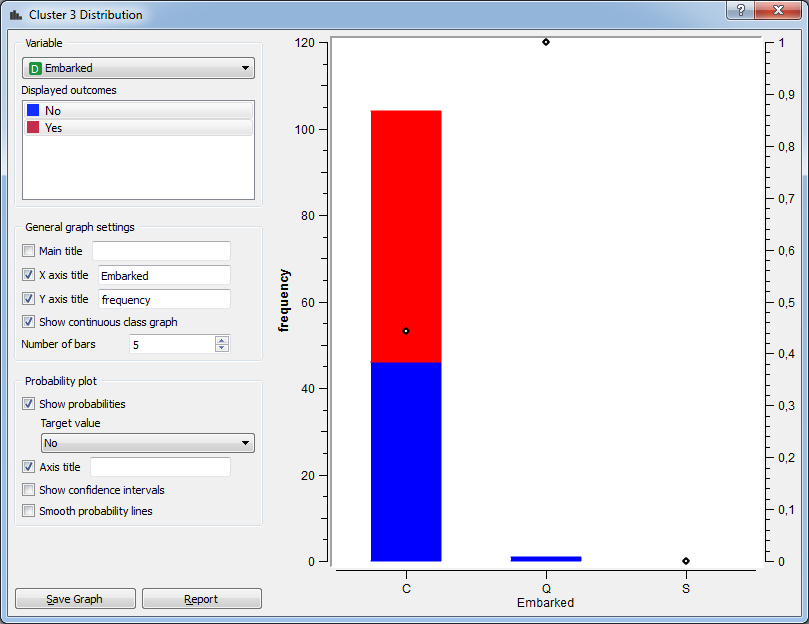
\includegraphics[scale=0.30]{ClusterDistribution/Cluster3/Embarked}
		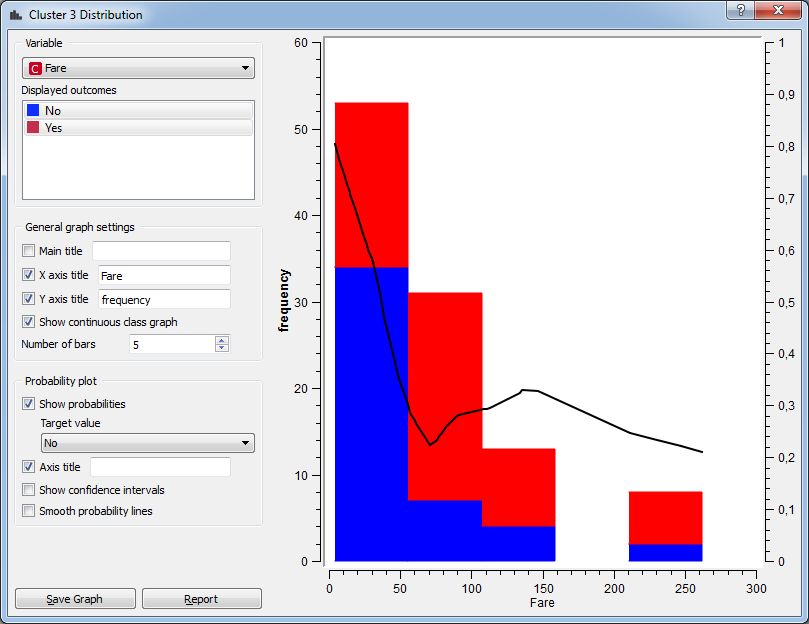
\includegraphics[scale=0.30]{ClusterDistribution/Cluster3/Fare}
	\end{center}
	\caption{Cluster 3}
	\label{ClusterThree}
\end{figure}


\subsubsection{Data validation}
10 fold cross validation
\clearpage
\section{Conclusion}
\subsection{Societal impact}
Time travellers could use this information to go on the titanic to have the adventure of a lifetime trying to use statistics to survive.

The classification tree could be used to predict the survival of people whose whereabouts were unknown.




\appendix
\begin{thebibliography}{9}

\bibitem{orange}
  \emph{Orange Data Mining},
  http://orange.biolab.si/,
  13-05-15
  
\bibitem{kaggleData}
	\emph{Kaggle Titanic data},
	https://www.kaggle.com/c/titanic,
	14-05-15
	
\bibitem{KMeans}
	\emph{K-Means Clustering},
	http://en.wikipedia.org/wiki/K-means\_clustering,
	14-05-15
\end{thebibliography}

\end{document}


